\documentclass{article}
\usepackage[utf8]{inputenc}
\usepackage{amsmath}
\usepackage{comment}
\usepackage{graphicx}
\usepackage{geometry}
 \geometry{
 a4paper,
 total={170mm,257mm},
 left=20mm,
 top=20mm,
 }

\title{\LARGE 3GPP LTE : Cramer Rao Lower Bound on TOA}
\author{Siddhant}
\date{May 2020}

\begin{document}

\maketitle
\section{\LARGE Position reference Sequence Based CRLB}

\subsection{CRLB Analysis : General Delay Estimation in AWGN}
Assume a signal $s(t)$ transmitted at time $0$ till $T_s$ from eNB and being received at UE from time $\tau_0$ till $T_s+\tau_0$, $T_s$ being symbol period. Received signal $x(t)$ can be expressed as follows:
$$x(t) = s(t - \tau_0) + w(t)$$

$w(t)$ is the White Gaussian Noise process with distribution $\sim \mathcal N (0, \sigma^2)$. Also, baseband signal $s(t)$ is band-limited to $f_{max}=B$.

Consider sampled version of $x(t)$ sampled at Nyquist Rate $2B = \frac{1}{\Delta}$. Sampled noise $w[n]$ will be independent. $x(n\Delta)$ will be non-zero only from time $\tau_0$ to $\tau_0 + T_s$. Mathematically, $x[n\Delta]$ can be expressed as follows:
$$x[n\Delta] = s[n\Delta - \tau_0] + w[n],$$
Assuming $\Delta$ to be small enough such that $\tau_0$ is some integral multiple of $\Delta$, $\frac{\tau_0}{\Delta} = n_0$.
Based on the final result of appendix $\mathbf{A}$, Cramer-Rao Lower Bound for delay $\tau_0$ can be given by the following expression:

$$
var(\hat{\tau_0}) \ge \frac{\sigma^2}{\sum^{n_0+N-1}_{n=n_0}(\frac{\partial s[n\Delta - \tau_0]}{\partial \tau_0 })^2} = \frac{\sigma^2}{\sum^{n_0+N-1}_{n=n_0}(\frac{\partial s(t)}{\partial t})| ^2 _{t=n\Delta - \tau_0}}
$$

\begin{equation} \label{eq1}
\LARGE
\boxed{var(\hat{\tau_0}) \ge \frac{\sigma^2}{\sum^{N-1}_{n=0}(\frac{\partial s(t)}{\partial t})| ^2 _{t=n\Delta}}}
\end{equation}
\\
The summation in the equ.(1) can be approximated to be integration since $\Delta$ is assumed to be very small and $n_0\Delta = \tau_0$. 
\begin{equation} \label{eq2} \LARGE
var(\hat{\tau_0}) \ge \frac{\sigma^2}{\frac{1}{\Delta} \int^{T_s}_{0}(\frac{\partial s(t)}{\partial t})^2 \partial t} = \boxed{\frac{\Delta. \sigma^2}{\int^{T_s}_{0}(\frac{\partial s(t)}{\partial t})^2 \partial t}}
\end{equation}

\begin{equation} \label{eq3} \LARGE
\boxed{var(\hat{\tau_0}) \ge \frac{N_0/2}{\int^{T_s}_{0}(\frac{\partial s(t)}{\partial t})^2 \partial t}}
\end{equation}

Observe that signal energy $\mathcal E = \int^{T_s}_{0}|s(t)|^2\partial t$ and define a quantity $\bar{F}^2$ as follows:
$$\bar{F}^2 = \frac{\int^{T_s}_{0}(\frac{\partial s(t)}{\partial t})^2 \partial t}{\int^{T_s}_{0}|s(t)|^2\partial t}$$
\\
Now, we can write equation.2 using $\mathcal E$ and $\bar{F}^2$ as follows:
\begin{equation} \label{eq4} \LARGE
\boxed{var(\hat{\tau_0}) \ge \frac{1}{\frac{\mathcal{E}}{N_0/2}\cdot \bar{F}^2} = \frac{1}{\mathbf{SNR} \cdot \bar{F}^2}}
\end{equation}
\\
This quantity $\bar{F}^2$ can be understood as Mean-Squared Bandwidth \footnote{Area under the curve $f^2$ weighted by transmitted signal's PSD $|S(f)|^2$ over $f \in (-\infty, \infty)$ will give squared bandwidth of $s(t)$. And, this squared bandwidth is divided by total signal power.} of the transmitted signal $s(t)$. This is also called Gabor Bandwidth. Using Fourier Transform's properties $\bar{F}^2$ can be written as follows:
\begin{equation} \label{eq5}
\LARGE
\boxed{\bar{F}^2 = \frac{\int^{\infty}_{-\infty}(2\pi f)^2|S(f)|^2\partial f}{\int^{\infty}_{-\infty}|S(f)|^2\partial f}}
\end{equation}
\\

\subsection{CRLB Derivation : PRS Based OFDM System}
A transmitted signal $s[n]$ can be written as inverse discrete fourier transform summation as follows:
$$s[n] = \sqrt{\frac{2C}{N}} \sum_{k \in N_a}d_k exp(j2\pi n k/N)$$
$N$ is the number of tones i.e. $12N_{RB}$, $N_a$ is the number of active tones on which the PRS symbols are loaded, $d_k$ are Gold Sequenced QAM symbols on $k^{th}$ tone, and $C$ is the total power in one OFDM Symbol of symbol period $T_s$, where $T_s = \frac{1}{\Delta f}$. $C$ can be expressed in terms of total signal energy and symbol period as follows:
$$C = \frac{\sum^{N-1}_{k=0}|X[k\Delta f]|^2}{T_s}$$
And, hence One Symbol Energy $\mathcal E_s$ can be defined as: $\mathcal E_s = C T_s$. Also, we note that $X[k \Delta f] = d_k$.
\\
Based on the analysis of CRLB for delay in previous section, we can write the CRLB for this PRS based OFDM system as follows:
\begin{equation} \label{eq6} \large
var(\hat{\tau}) \ge \frac{\sigma^2}{\{\sum^{N-1}_{k=0}|X[k\Delta f]|^2\}\cdot \bar{F}^2}
\end{equation}
\\
For any OFDM System, Mean-Squared Bandwidth ($\bar{F}^2$) can be approximated by the following expression:
\begin{equation} \label{eq7} \large
\bar{F}^2 = \frac{\sum^{N-1}_{k=0}(2\pi k\Delta f)^2|X[k\Delta f]|^2}{\sum^{N-1}_{k=0}|X[k\Delta f]|^2} = \frac{\sum^{N-1}_{k=0}(2\pi k\Delta f)^2|d_k|^2}{\sum^{N-1}_{k=0}|d_k|^2}
\end{equation}
\\
If we can assume that $d_k$ will be one of the QAM symbols picked from the set: $\{ \frac{1}{\sqrt{2}} (1+j) , \frac{1}{\sqrt{2}} (1-j), \frac{1}{\sqrt{2}} (-1+j), \frac{1}{\sqrt{2}} (-1-j) \}$, then $|d_k|^2 = 1$. Also approximate $\sum^{N-1}_{k=0}k^2 \approx \frac{2N^3}{6}$ for large $N$. Hence expression for $\bar{F}^2$ can be simplified to the following:
\\
\begin{equation} \label{eq8} \LARGE
\bar{F}^2 = \frac{(2\pi \Delta f)^2 \sum^{N-1}_{k=0}k^2}{N} \approx  \frac{4\pi^2}{3}(N\Delta f)^2
\end{equation}
\\
Using equ.(2) and equ.(8), we can write the CRLB for TOA for PRS based OFDM system as follows:
\\
$$var(\hat{\tau}) \ge \frac{\sigma^2/(N\Delta f)}{\frac{4\pi^2}{3}(N\Delta f)^2 \cdot \sum^{N-1}_{k=0}|X[k\Delta f]|^2}$$ 
\\
$$ var(\hat{\tau}) \ge \frac{\sigma^2/(N\Delta f)}{\frac{4\pi^2}{3}(N\Delta f)^2 \cdot \sum^{N-1}_{k=0}|d_k|^2} = \frac{1}{\frac{4\pi^2}{3}(N\Delta f)^2 \cdot \frac{\sum_{k}|d_k|^2}{\sigma^2/(N\Delta f)}}$$
\\
Notice that the quantity $\frac{\sum_{k}|d_k|^2}{\sigma^2/(N\Delta f)}$ is the Post-Correlation SNR. Because, when we correlate the received symbols with the Gold Sequence of PRS, what we will have as aggregate signal energy, is : $\sum_{k}|d_k|^2$, and we know that noise power in the total OFDM Bandwidth $2B = 12N_{RB}\Delta f$ is nothing but $\sigma^2 = N_0/2.2B = N_0B$, where $N_0/2$ is double sided noise PSD. Hence, $\sigma^2/(N\Delta f)$ is Noise-Energy. So, we can write $\frac{\sum_{k}|d_k|^2}{\sigma^2/(N\Delta f)} = {SNR}_{PostCorr}$. We can also interpret the quantity, $\frac{\sum_{k}|d_k|^2}{1/(N\Delta f)}$ as post-correlation signal power and $\sigma^2 = N_0/2$ is the Noise Power, and hence, $\frac{\sum_{k}|d_k|^2}{\sigma^2/(N\Delta f)} = {SNR}_{PostCorr}$  . The final CRLB expression for this PRS(Pilot) based delay estimation in OFDM Based 4GLTE or 5GNR system can be given by the following:
\\
\begin{equation} \label{eq9}
\LARGE
\boxed{CRLB(\hat{\tau}) = var(\hat{\tau}) \ge \frac{1}{\frac{4\pi^2}{3} \ (N\Delta f)^2 \ {SNR}_{PostCorr}} }
\end{equation}

\begin{figure}[h]
\caption{Cramer-Rao Lower Bound and 5G PRS in AWGN Channel}
\centering
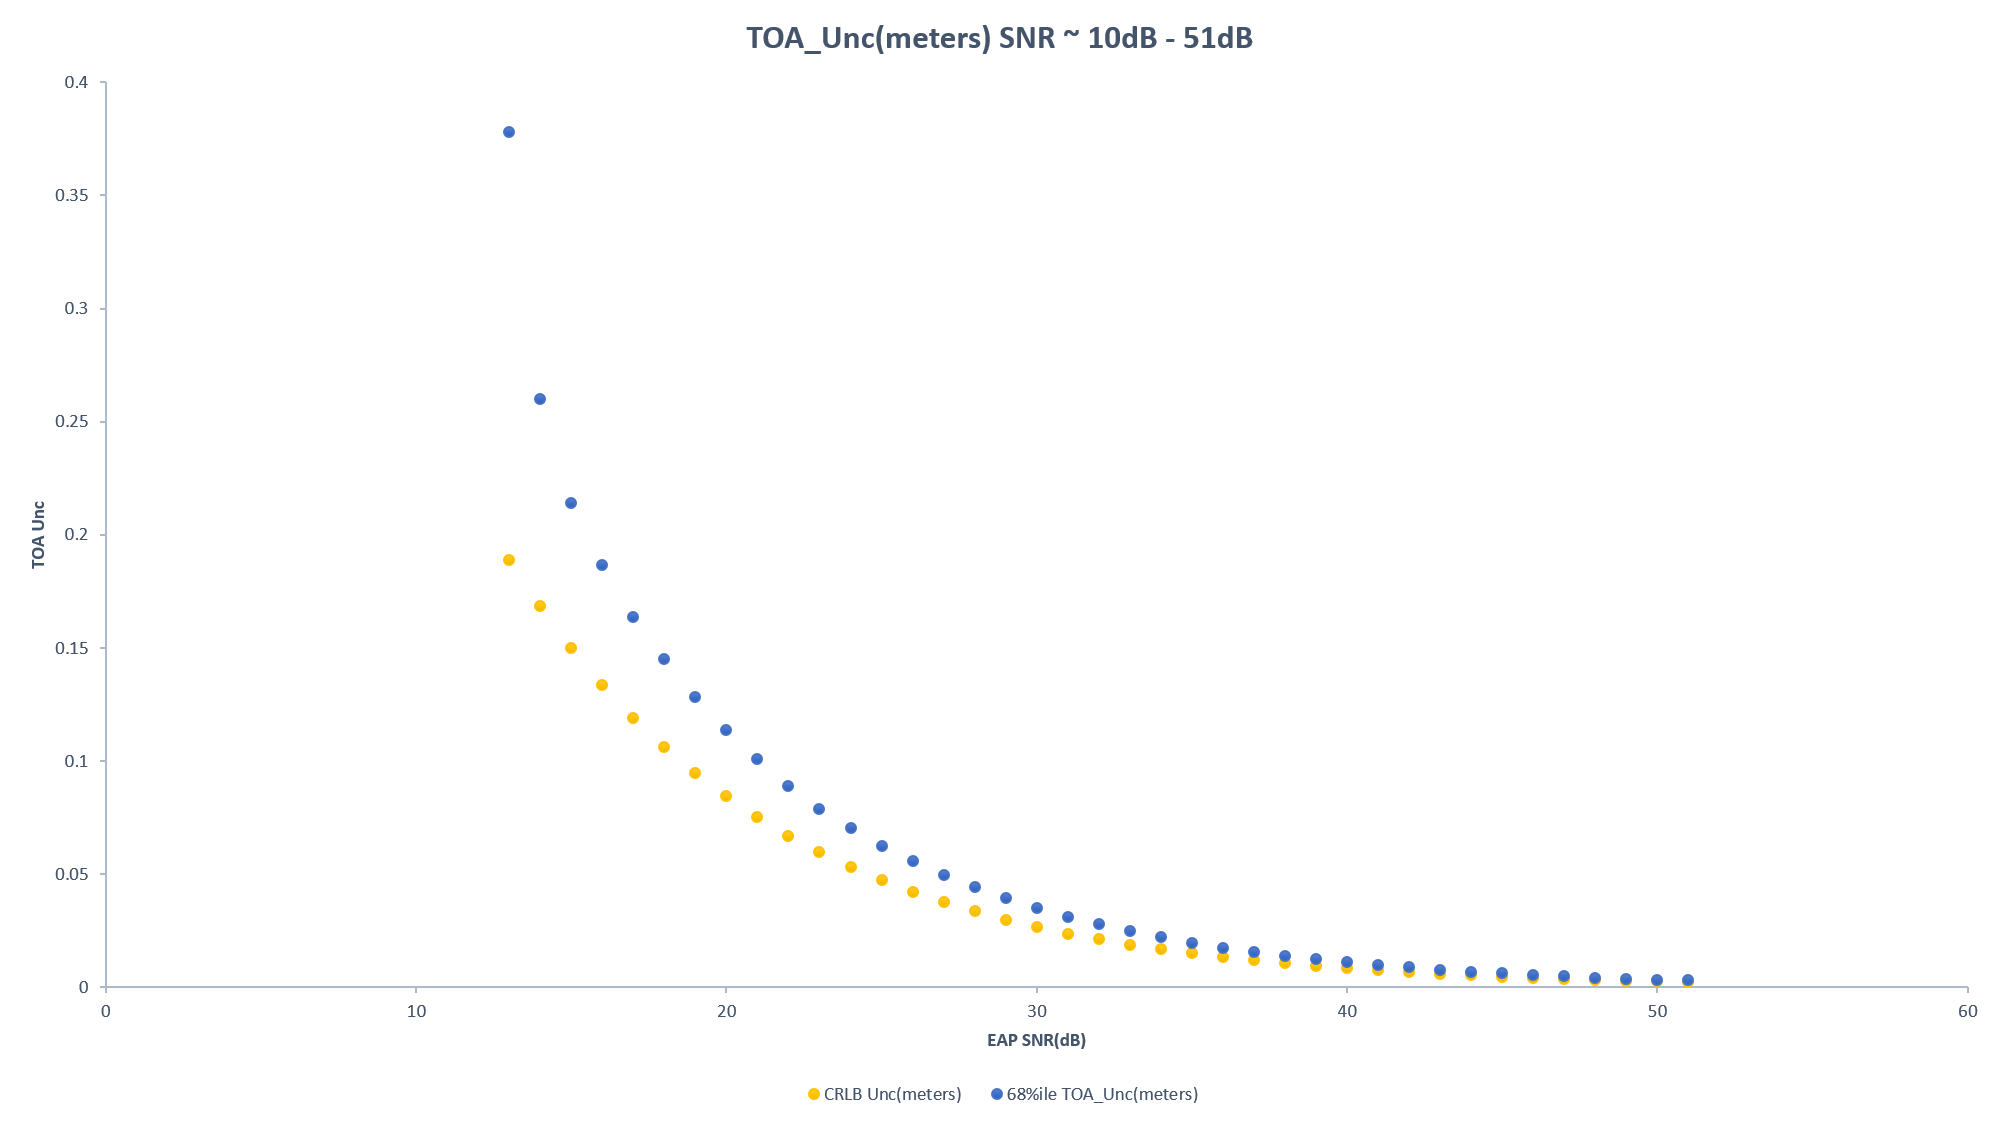
\includegraphics[scale=0.5]{CRLB_toa}
\end{figure}
\begin{comment}
\newpage
\section{Alternative : CRLB for OFDM Based Systems}
\subsection{Derivation: Fisher Information}
$s(t)$ is the OFDM wave being transmitted by Reference Cell. $\tau$ is the time delay and channel is assumed to be $1$. Received Samples can be given by the following :
\\
$$y[n] = s(nT_s - \tau) + z[n],$$where z[n] are iid AWGN noise samples with mean $0$ and variance $\sigma^2$.  
Joint Conditional PDF of $\mathbf y|\tau$ can be given by the following:
$$p(\mathbf y|\tau) = \frac{1}{(\pi \sigma^2)^N} .exp(-\frac{1}{\sigma^2}\sum^{N}_{n=1}(s(n T_s - \tau) - y[n])^2)$$
\\
And log likelihood will become :
\\
$$ln(p(\mathbf y|\tau)) = -N ln(\pi \sigma^2) -\frac{1}{\sigma^2}\sum^{N}_{n=1}(s(nT_s - \tau) - y[n])^2$$
\\
Fisher Information $\mathbf J(\tau)$ will then be given by:
\\
$$\mathbf{J}(\tau) = \mathbf E\{ - \mathbf{\frac{d^2}{d^2\tau}}ln((p(\mathbf y|\tau)) \}$$
\\
Simplify the above to get :
\\
$$\mathbf{J}(\tau) = \frac{2}{sigma^2}\sum^{N}_{n=1}\mathbf{\frac{d}{d\tau}}s(n T_s - \tau).\mathbf{\frac{d}{d\tau}}s^*(n T_s - \tau)$$
\\
Since, $s(t) = \frac{1}{\sqrt{N}}\sum^{\frac{N}{2} - 1}_{k=-\frac{N}{2}}S[k]e^{j2\pi k\Delta F t}$, where $\Delta F$ is subcarrier spacing of OFDM system. Hence, $s(n T_s - \tau) = \frac{1}{\sqrt{N}}\sum^{\frac{N}{2} - 1}_{k=-\frac{N}{2}}S[k]e^{j2\pi k\Delta F (n T_s - \tau)}$. Substitute this $s(n T_s - \tau)$ in the above equation to get : 
\\
$$\mathbf{J}(\tau) = \frac{2}{N.\sigma^2} \sum^{N}_{n=1}\{\frac{d}{d\tau}\sum^{\frac{N}{2} - 1}_{k=-\frac{N}{2}}S[k]e^{j2\pi k\Delta F (n T_s - \tau)}\}.\{\frac{d}{d\tau}\sum^{\frac{N}{2} - 1}_{l=-\frac{N}{2}}S[k]e^{j2\pi l\Delta F (n T_s - \tau)}\}$$
\\
After carrying out differentiation and taking all terms which are not running in the sum out of the summation, we get the following :
$$\mathbf{J}(\tau) = \frac{2}{N\sigma^2}(-j2\pi \Delta F).(j2\pi \Delta F)\sum^{N}_{n=1} \{\sum^{\frac{N}{2} - 1}_{k=-\frac{N}{2}}k S[k]e^{j2\pi \Delta F k n T_s}.\sum^{\frac{N}{2} - 1}_{l=-\frac{N}{2}}l S*[l]e^{-j2\pi \Delta F l n T_s}\}$$
\\
Use orthogonality of Fourier Basis and assume $S[k] = 1$, to get the following:
\\
$$\mathbf{J}(\tau) = \frac{8\pi^2 \Delta F^2}{N\sigma^2} \sum^{N}_{n=1} \sum^{\frac{N}{2} - 1}_{k=-\frac{N}{2}}N k^2 = \frac{8\pi^2 \Delta F^2}{\sigma^2} \sum^{N}_{n=1} \sum^{\frac{N}{2} - 1}_{k=-\frac{N}{2}}k^2 = \frac{8\pi^2 \Delta F^2 N}{\sigma^2}\sum^{\frac{N}{2} - 1}_{k=-\frac{N}{2}}k^2$$
\\
Computing $\sum^{\frac{N}{2} - 1}_{k=-\frac{N}{2}}k^2$ by substituting $m=k+\frac{N}{2}$, gives the following :
\\
$$\sum^{N-1}_{m=0}(m-\frac{N}{2})^2 = \frac{N^3}{12} + \frac{N}{6} \approx \frac{N^3}{12}$$
\\
Finally, plug this approximated sum into Fisher Information sum to get the following :
\\
$$\mathbf{J}(\tau) = \frac{8\pi^2 \Delta F^2 N}{\sigma^2}\sum^{\frac{N}{2} - 1}_{k=-\frac{N}{2}}k^2 \approx \frac{8\pi^2 \Delta F^2 N}{\sigma^2} \frac{N^3}{12},$$
\\
We know that Bandwidth of OFDM is $\Delta F.N$, hence $(\Delta F . N)^2$ can be considered as Squared Bandwidth. Also We have considered $|S[k]|^2 = 1$, which will mean Pre-Correlation Signal Power is 1. If instead Pre-Correlation Signal Power was a constant $P$, then Post-Correlation signal power would have been $N.P$. And then the Fisher Information expression becomes :
\\
$$\mathbf{J}(\tau) = \frac{2\pi^2 (\Delta F.N)^2}{3}. \frac{N^2 P}{\sigma^2} = N. \frac{2\pi^2}{3} (\Delta F.N)^2 SNR_{corr}$$
\\
\subsection{CRLB : Expression}
As, CRLB on uncertainty of the estimated parameter $\tau$ is lower bounded by reciprocal of Fisher Information, CRLB can be given by following:
$$var(\hat{\tau}) \ge \frac{1}{\mathbf J(\tau)},$$
$$or, var(\hat{\tau}) \ge \frac{3}{2N\pi^2}\frac{1}{(\Delta F.N)^2}.\frac{1}{SNR_{corr}}$$
\end{comment}

\newpage
\appendix
\section{CRLB : Signal($s[n;\theta]$) in White Gaussian Noise}
Assume the observations $x[n]$ to be:
\\
$$x[n] = s[n;\theta] + w[n],$$
\\
$w[n]$ are iid noise samples distributed $\sim \mathcal{N}(0, \sigma^2)$. Joint PDF of $N$ independent observations $p(\mathbf x; \theta)$ and log-likelihood function will be given by:
\\
$$p(\mathbf x; \theta) = \frac{1}{(\sqrt{2\pi \sigma^2})^N} \cdot exp(-\frac{1}{2\sigma^2}\sum^{N-1}_{n=0}(x[n] - s[n;\theta])^2)$$
$$\ln{p(\mathbf x;\theta)} = -\frac{N}{2}\ln{2\pi \sigma^2} - \frac{1}{2\sigma^2}\sum^{N-1}_{n=0}(x[n] - s[n;\theta])^2$$
\\
Differentiating with respect to $\theta$, we get the following:
\\
$$\frac{\partial \ln{p(\mathbf x; \theta)}}{\partial \theta} = \frac{1}{\sigma^2}\sum^{N-1}_{n=0}\frac{\partial s[n;\theta]}{\partial \theta}(x[n] - s[n;\theta])$$
\\
It can be verified that the regularity condition($\mathcal{E}\{ \frac{\partial \ln{p(\mathbf x; \theta)}}{\partial \theta} \} = 0, \forall \theta$), is satisfied. Differentiating again with respect to $\theta$, we get the following:
$$\frac{\partial ^2 \ln{p(\mathbf x; \theta)}}{\partial ^2 \theta} = \frac{1}{\sigma^2}\sum^{N-1}_{n=0}(\frac{\partial ^2s[n;\theta]}{\partial ^2\theta}(x[n] - s[n;\theta]) - (\frac{\partial s[n;\theta]}{\partial \theta})^2)$$
This leads to Fisher information $\mathbf I (\theta) = -\mathbf E \{ \frac{\partial ^2\ln{p(\mathbf x; \theta)}}{\partial ^2\theta} \}$:
\\
$$\mathbf I(\theta) = \frac{1}{\sigma^2}\sum^{N-1}_{n=0}(\frac{\partial s[n;\theta]}{\partial \theta} )^2 $$
\\
Cramer Rao Lower bound on estimation of unknown parameter $\theta$ is given by the reciprocal of Fisher information $\mathbf{I}(\theta)$, so in this case of general signal parametrized by unknown component $\theta$ is given as follows:
\\
\begin{equation} \label{eqA}
\LARGE
\boxed {var(\hat{\theta}) \ge \frac{\sigma^2}{ \sum^{N-1}_{n=0} (\frac{\partial s[n;\theta]}{\partial \theta} )^2}}
\end{equation}

\newpage
\nocite{*}
\bibliography{myRef}
\bibliographystyle{ieeetr}

\end{document}
